\documentclass[aspectratio=169,10pt]{beamer}
\usepackage{amsmath,amssymb,amsthm}
\usepackage{mathtools}
\usepackage{tikz}
\usetikzlibrary{calc,angles,quotes,decorations.markings,arrows.meta,shapes.geometric,positioning,fit,backgrounds,patterns}
\usepackage{xcolor}
\usepackage{graphicx}
\usepackage{microtype}
\usepackage{hyperref}
\definecolor{morleydark}{RGB}{45,35,55}
\definecolor{morleymain}{RGB}{120,80,140}
\definecolor{morleyaccent}{RGB}{200,140,80}
\definecolor{morleylight}{RGB}{245,240,235}
\definecolor{morleygold}{RGB}{190,150,70}
\definecolor{morleyblue}{RGB}{75,100,150}
\definecolor{morleygreen}{RGB}{85,130,95}
\definecolor{morleyred}{RGB}{155,75,75}
\definecolor{morleypurple}{RGB}{130,90,140}

\setbeamercolor{normal text}{fg=morleydark,bg=white}
\setbeamercolor{frametitle}{fg=morleymain,bg=morleylight}
\setbeamercolor{title}{fg=morleydark}
\setbeamercolor{subtitle}{fg=morleymain}
\setbeamercolor{structure}{fg=morleymain}
\setbeamercolor{alerted text}{fg=morleyred}
\setbeamercolor{example text}{fg=morleygreen}
\setbeamercolor{block title}{fg=white,bg=morleymain}
\setbeamercolor{block body}{fg=morleydark,bg=morleylight}
\setbeamercolor{item}{fg=morleymain}

\setbeamertemplate{itemize item}[circle]
\setbeamertemplate{itemize subitem}[triangle]
\setbeamertemplate{navigation symbols}{}
\setbeamertemplate{footline}[frame number]

\setbeamertemplate{frametitle}{\vspace{0.2cm}\insertframetitle\par\vspace{-0.1cm}{\color{morleyaccent}\rule{0.5\textwidth}{0.6pt}}}

\title{\textbf{Morley's Theorem}}
\subtitle{\large\textit{All Roads Lead to Geometry}}
\author{Sanatan Kumar Gupta}
\date{16/04/2026}

\begin{document}

\begin{frame}[plain]
\begin{tikzpicture}[remember picture,overlay]
  \fill[morleylight] (current page.south west) rectangle (current page.north east);
  \node[opacity=0.1] at ($(current page.center)+(4cm,0.5cm)$) {\begin{tikzpicture}[scale=1.8]\draw[line width=5pt,morleymain] (0,0)--(3,0)--(1.5,2.598)--cycle;\end{tikzpicture}};
\end{tikzpicture}
\vspace{1.5cm}
\begin{center}
  {\Huge\textcolor{morleymain}{\textbf{Morley's Theorem}}}\\[0.3cm]
  {\Large\textcolor{morleyaccent}{\textit{All Roads Lead to Geometry}}}\\[0.8cm]
  {\normalsize\textcolor{morleydark!80}{\textbf{Sanatan Kumar Gupta}}}\\[0.1cm]
  {\small\textcolor{morleydark!60}{19/04/2026}}\\[0.8cm]
  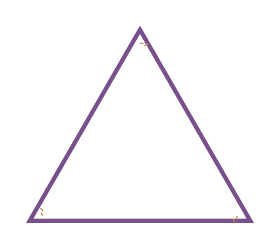
\begin{tikzpicture}[scale=0.7]
    \draw[line width=1.5pt,morleymain] (0,0)--(4,0)--(2,3.464)--cycle;
    \foreach \a/\b/\c in {0/0/20,4/0/160,2/3.464/270} {
      \draw[morleyaccent,line width=0.4pt] (\a,\b) ++(\c:0.25) arc (\c:\c+15:0.25);
      \draw[morleyaccent,line width=0.4pt] (\a,\b) ++(\c+15:0.3) arc (\c+15:\c+30:0.3);
    }
  \end{tikzpicture}
\end{center}
\end{frame}

\begin{frame}{Outline of the Journey}
\begin{columns}[T]
\begin{column}{0.55\textwidth}
\vspace{0.2cm}
\begin{itemize}
  \setlength\itemsep{0.5em}
  \item \textbf{\textcolor{morleymain}{Introduction}}
  \begin{itemize}\small
    \item The Theorem
  \end{itemize}
  \vspace{0.2cm}
  \item \textbf{\textcolor{morleymain}{Five Lenses on Morley's Theorem}}
  \begin{itemize}\small
    \item Trigonometric Proof
    \item Algebraic Proof 
    \item Synthetic Proof 
    \item Group Theory Proof 
    \item Circle Intersection Proof
  \end{itemize}
  \vspace{0.2cm}
  \item \textbf{\textcolor{morleymain}{Conclusion}}
  \begin{itemize}\small
    \item Beyond the Proofs
    \item References
  \end{itemize}
\end{itemize}
\end{column}
\begin{column}{0.45\textwidth}
\vspace{0.8cm}
\centering
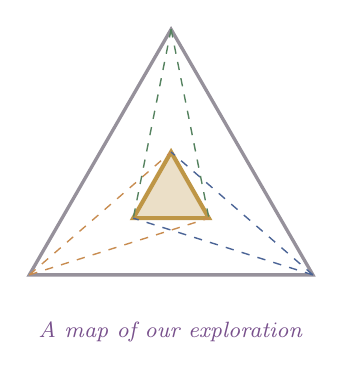
\begin{tikzpicture}[scale=1.2]
  \coordinate (A) at (0,0); \coordinate (B) at (3,0); \coordinate (C) at (1.5,2.598);
  \draw[line width=1.2pt,morleydark!50] (A)--(B)--(C)--cycle;
  \coordinate (M1) at (1.1,0.6); \coordinate (M2) at (1.9,0.6); \coordinate (M3) at (1.5,1.3);
  \fill[morleygold!30] (M1)--(M2)--(M3)--cycle;
  \draw[line width=1.5pt,morleygold] (M1)--(M2)--(M3)--cycle;
  \draw[morleyaccent,line width=0.5pt,dashed] (A)--(M2); \draw[morleyaccent,line width=0.5pt,dashed] (A)--(M3);
  \draw[morleyblue,line width=0.5pt,dashed] (B)--(M1); \draw[morleyblue,line width=0.5pt,dashed] (B)--(M3);
  \draw[morleygreen,line width=0.5pt,dashed] (C)--(M1); \draw[morleygreen,line width=0.5pt,dashed] (C)--(M2);
  \node[font=\footnotesize,morleymain] at (1.5,-0.6) {\textit{A map of our exploration}};
\end{tikzpicture}
\end{column}
\end{columns}
\end{frame}


\begin{frame}{The Theorem}
\vspace{0.5cm}
\begin{columns}
\begin{column}{0.4\textwidth}
\begin{block}{\normalsize Morley's Trisector Theorem}
\normalsize
The three points of intersection of the \textbf{adjacent trisectors} of the angles of any triangle form an \textbf{equilateral triangle}.
\end{block}
\end{column}
\begin{column}{0.6\textwidth}
\centering
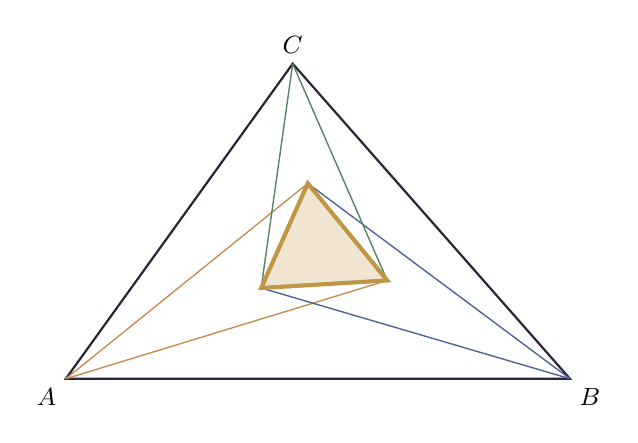
\begin{tikzpicture}[scale=1.6]
  \coordinate (A) at (0,0); \coordinate (B) at (4,0); \coordinate (C) at (1.8,2.5);
  \coordinate (M1) at (1.55,0.72); \coordinate (M2) at (2.55,0.78); \coordinate (M3) at (1.92,1.55);
  \draw[line width=0.8pt,morleydark] (A)--(B)--(C)--cycle;
  \draw[morleyaccent,line width=0.5pt] (A)--(M2); \draw[morleyaccent,line width=0.5pt] (A)--(M3);
  \draw[morleyblue,line width=0.5pt] (B)--(M1); \draw[morleyblue,line width=0.5pt] (B)--(M3);
  \draw[morleygreen,line width=0.5pt] (C)--(M1); \draw[morleygreen,line width=0.5pt] (C)--(M2);
  \fill[morleygold!25] (M1)--(M2)--(M3)--cycle;
  \draw[line width=1.5pt,morleygold] (M1)--(M2)--(M3)--cycle;
  \node[below left,font=\small] at (A) {$A$}; \node[below right,font=\small] at (B) {$B$}; \node[above,font=\small] at (C) {$C$};
\end{tikzpicture}
\end{column}
\end{columns}
\end{frame}

% =====================================================
% PROOF 1: TRIGONOMETRIC PROOF (PART 1)
% =====================================================
\begin{frame}{Proof 1: Trigonometric Proof (Part 1)}
\begin{columns}[T]
\begin{column}{0.54\textwidth}
\small
\textbf{Law of Sines Computation}
\vspace{0.1cm}

Let $\angle A = 3\alpha, \angle B = 3\beta, \angle C = 3\gamma$, so $\alpha+\beta+\gamma=60^\circ$. Assume the circumradius of $\triangle ABC$ is $1$. Then $BC=2\sin(3\alpha)$.

\vspace{0.1cm}
In $\triangle BPC$, the Law of Sines gives:
\[ \frac{BP}{\sin\gamma} = \frac{BC}{\sin(180^\circ-\beta-\gamma)} = \frac{2\sin(3\alpha)}{\sin(60^\circ-\alpha)} \]
The triple angle identity $\sin(3\alpha) = 4\sin\alpha\sin(60^\circ+\alpha)\sin(60^\circ-\alpha)$ cancels the denominator:
\begin{align*}
BP &= \frac{8\sin\alpha\sin(60^\circ+\alpha)\sin(60^\circ-\alpha)\sin\gamma}{\sin(60^\circ-\alpha)} \\
   &= 8\sin\alpha\sin\gamma\sin(60^\circ+\alpha)
\end{align*}
By symmetry, in $\triangle ARB$, we find:
\[ BR = 8\sin\gamma\sin\alpha\sin(60^\circ+\gamma) \]
\end{column}
\begin{column}{0.46\textwidth}
\centering
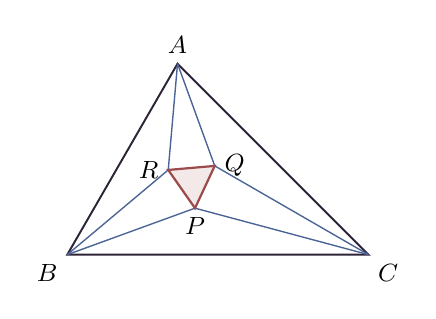
\begin{tikzpicture}[scale=0.85]
  \coordinate (B) at (0,0);
  \coordinate (C) at (4.5,0);
  \coordinate (Btop) at ($(B)+(60:5)$);
  \coordinate (Ctop) at ($(C)+(135:5)$);
  \coordinate (A) at (intersection of B--Btop and C--Ctop);

  \coordinate (Br) at ($(B)+(40:4)$);
  \coordinate (Bp) at ($(B)+(20:4)$);
  \coordinate (Cp) at ($(C)+(165:4)$);
  \coordinate (Cq) at ($(C)+(150:4)$);
  \coordinate (Ar) at ($(A)+(265:4)$);
  \coordinate (Aq) at ($(A)+(290:4)$);

  \coordinate (R) at (intersection of B--Br and A--Ar);
  \coordinate (P) at (intersection of B--Bp and C--Cp);
  \coordinate (Q) at (intersection of A--Aq and C--Cq);

  \draw[line width=0.7pt,morleydark] (A) -- (B) -- (C) -- cycle;
  
  \draw[morleyblue,line width=0.5pt] (A) -- (R);
  \draw[morleyblue,line width=0.5pt] (A) -- (Q);
  \draw[morleyblue,line width=0.5pt] (B) -- (R);
  \draw[morleyblue,line width=0.5pt] (B) -- (P);
  \draw[morleyblue,line width=0.5pt] (C) -- (P);
  \draw[morleyblue,line width=0.5pt] (C) -- (Q);

  \fill[morleyred!12] (P) -- (Q) -- (R) -- cycle;
  \draw[morleyred,line width=0.8pt] (P) -- (Q) -- (R) -- cycle;
  
  \node[above,font=\small] at (A) {$A$};
  \node[below left,font=\small] at (B) {$B$};
  \node[below right,font=\small] at (C) {$C$};
  \node[left,font=\small] at (R) {$R$};
  \node[below,font=\small] at (P) {$P$};
  \node[right,font=\small] at (Q) {$Q$};
\end{tikzpicture}

\end{column}
\end{columns}
\end{frame}

\begin{frame}{Proof 1: Trigonometric Proof (Part 2)}
\begin{columns}[T]
\begin{column}{0.54\textwidth}
\small
\textbf{Law of Cosines \& Reference Triangle}

In $\triangle BPR$, we apply the Law of Cosines:
\[ PR^2 = BP^2 + BR^2 - 2(BP)(BR)\cos\beta \]
Substituting our expressions for $BP$ and $BR$:
\begin{align*}
PR^2 &= 64\sin^2\alpha\sin^2\gamma \big[ \sin^2(60^\circ+\alpha) \\
     &\quad + \sin^2(60^\circ+\gamma) \\
     &\quad - 2\sin(60^\circ+\alpha)\sin(60^\circ+\gamma)\cos\beta \big]
\end{align*}

\textbf{Key Step:} Consider a reference triangle with angles $60^\circ+\alpha$, $60^\circ+\gamma$, and $\beta$ (which sum to $180^\circ$). 
If its circumradius is $1$, its sides are $2\sin(60^\circ+\alpha)$, $2\sin(60^\circ+\gamma)$, and $2\sin\beta$.

Applying the Law of Cosines to this reference triangle reveals that the bracketed term is exactly $\sin^2\beta$!
\end{column}
\begin{column}{0.46\textwidth}
\small
Thus, the expression collapses to:
\[ PR^2 = 64\sin^2\alpha\sin^2\gamma\sin^2\beta \]
\[ \Rightarrow PR = 8\sin\alpha\sin\beta\sin\gamma \]

This expression is symmetric in $\alpha$, $\beta$, $\gamma$. By symmetry, $PQ = QR = 8\sin\alpha\sin\beta\sin\gamma$.

\begin{center}
\textcolor{morleymain}{\textbf{Therefore, $PR = PQ = QR$.}} \\
\textcolor{morleyaccent}{\textbf{$\triangle PQR$ is equilateral!}}
\end{center}

\centering
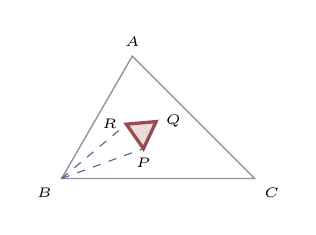
\begin{tikzpicture}[scale=0.7]
  \coordinate (B) at (0,0);
  \coordinate (C) at (3.5,0);
  \coordinate (Btop) at ($(B)+(60:4)$);
  \coordinate (Ctop) at ($(C)+(135:4)$);
  \coordinate (A) at (intersection of B--Btop and C--Ctop);

  \coordinate (Br) at ($(B)+(40:3)$); \coordinate (Bp) at ($(B)+(20:3)$);
  \coordinate (Cp) at ($(C)+(165:3)$); \coordinate (Cq) at ($(C)+(150:3)$);
  \coordinate (Ar) at ($(A)+(265:3)$); \coordinate (Aq) at ($(A)+(290:3)$);

  \coordinate (R) at (intersection of B--Br and A--Ar);
  \coordinate (P) at (intersection of B--Bp and C--Cp);
  \coordinate (Q) at (intersection of A--Aq and C--Cq);

  \draw[line width=0.5pt,morleydark!50] (A) -- (B) -- (C) -- cycle;
  
  \draw[morleyblue,line width=0.4pt,dashed] (B) -- (P);
  \draw[morleyblue,line width=0.4pt,dashed] (B) -- (R);
  
  \fill[morleyred!20] (P) -- (Q) -- (R) -- cycle;
  \draw[morleyred,line width=1.2pt] (P) -- (Q) -- (R) -- cycle;
  
  \node[above,font=\tiny] at (A) {$A$};
  \node[below left,font=\tiny] at (B) {$B$};
  \node[below right,font=\tiny] at (C) {$C$};
  \node[left,font=\tiny] at (R) {$R$};
  \node[below,font=\tiny] at (P) {$P$};
  \node[right,font=\tiny] at (Q) {$Q$};
\end{tikzpicture}
\end{column}
\end{columns}
\end{frame}

% =====================================================
% PROOF 2: ALGEBRAIC PROOF (PART 1)
% =====================================================
\begin{frame}{Proof 2: Algebraic Proof (Part 1)}
\begin{columns}[T]
\begin{column}{0.54\textwidth}
\small
\textbf{Turns on the Unit Circle}
\vspace{0.1cm}

We represent points as \textit{turns} (complex numbers with $|t|=1$, so $t^* = 1/t$).
Let $\omega = e^{2\pi i/3}$. A key property is that $\triangle pqr$ is equilateral if and only if:
\[ p + \omega q + \omega^2 r = 0 \quad (\text{or with } \omega \leftrightarrow \omega^2) \]

\textbf{The Setup:} Let the circumcircle of $\triangle ABC$ be the unit circle $U$. We assign the vertices $A, B, C$ the affixes $a^3, b^3, c^3$.

The points of trisection of the arcs $AB, BC, CA$ are elegantly given by the turn products:
\[ a^2b, ab^2; \quad b^2c, bc^2; \quad \omega c^2a, \omega^2 ca^2 \]
The interior trisectors of the triangle correspond to chords connecting these specific points on $U$.
\end{column}
\begin{column}{0.55\textwidth}
\centering
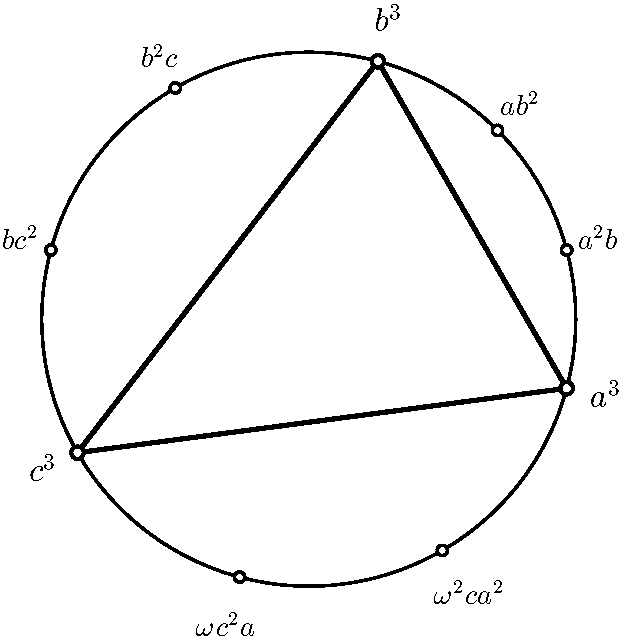
\includegraphics[width=0.75\linewidth]{figure4.pdf}
\end{column}
\end{columns}
\end{frame}

\begin{frame}{Proof 2: Algebraic Proof (Part 2)}
\begin{columns}[T]
\begin{column}{0.54\textwidth}
\small
\textbf{Chord Intersections}

The standard equation of a chord joining turns $t, u$ is $z + tuz^* = t+u$.
The Morley vertex $x$ is the intersection of chords $(ab^2, c^3)$ and $(b^3, \omega c^2 a)$.

Solving the system:
\begin{align*}
  x + ab^2c^3 x^* &= ab^2 + c^3 \\
  x + \omega ab^3c^2 x^* &= \omega ac^2 + b^3
\end{align*}
Subtracting yields:
\[ a^2b^2c^2 x^* = \omega^2(ab^2 \!-\! a^2b) + ac^2 \!-\! \omega a^2c + \omega abc \]
By cyclically permuting $a, b, c$, we obtain similar expressions for $y^*$ and $z^*$.
\end{column}
\begin{column}{0.46\textwidth}
\small
\textbf{Symmetry \& Conclusion}

Summing the cyclic expressions:
\[ x^* + \omega^2 y^* + \omega z^* = 0 \]
Taking the complex conjugate (since $\omega^* = \omega^2$):
\[ x + \omega y + \omega^2 z = 0 \]
This is exactly the condition for $\triangle xyz$ to be equilateral!

\centering
\includegraphics[width=0.53\linewidth]{figure6.pdf}
\end{column}
\end{columns}
\end{frame}


% =====================================================
% PROOF 3: SYNTHETIC PROOF (PART 1)
% =====================================================
\begin{frame}{Proof 3: Synthetic Proof (Part 1)}
\begin{columns}[T]
\begin{column}{0.45\textwidth}
\small
\textbf{Defining the Seven Pieces}
\vspace{0.1cm}

Conway's proof reverses the theorem: start with an equilateral triangle and build $\triangle ABC$ from 7 pieces.

Let $\alpha \!=\! A/3, \beta \!=\! B/3, \gamma \!=\! C/3$, so $\alpha \!+\! \beta \!+\! \gamma \!=\! 60^\circ$.
Define $\theta^* \!=\! \theta + 60^\circ$ and $\theta^{**} \!=\! \theta + 120^\circ$.

We define the following triangles (their angles sum to $180^\circ$):
\begin{itemize}\footnotesize
  \item \textbf{1 Central Equilateral:} $0^*, 0^*, 0^*$. Scaled to side-length 1.
  \item \textbf{3 Abutting Triangles:} e.g., $\alpha, \beta^*, \gamma^*$. Scaled so the side opposite $\alpha$ is 1.
  \item \textbf{3 Spoke Triangles:} e.g., $\alpha^{**}, \beta, \gamma$. (Scaling defined on next slide).
\end{itemize}
These 7 pieces are our building blocks.
\end{column}
\begin{column}{0.55\textwidth}
\centering
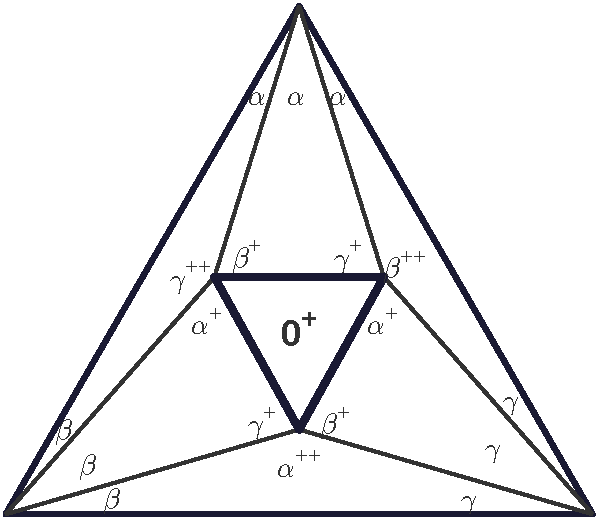
\includegraphics[width=0.75\linewidth]{figure.pdf}
\end{column}
\end{columns}
\end{frame}

\begin{frame}{Proof 3: Synthetic Proof (Part 2)}
\begin{columns}[T]
\begin{column}{0.54\textwidth}
\small
\textbf{Sizing the Spoke Triangles}
\vspace{0.1cm}

We must guarantee the pieces fit together. Consider the spoke triangle $PB'C'$ with angles $\alpha^{**}$ at $P$, $\beta$ at $B'$, and $\gamma$ at $C'$.

Fix points $Y$ and $Z$ on the line $B'C'$ such that the angles $\angle PYB'$ and $\angle PZC'$ equal $\alpha^*$. 

Because $\angle B'PY = 180^\circ - \beta - \alpha^* = \gamma^*$, the sub-triangle $\triangle B'PY$ has angles $\beta, \alpha^*, \gamma^*$. This makes it strictly similar to our abutting triangle!

We scale the spoke triangle so that $PY = PZ = 1$. Now the side $PY$ perfectly matches the side length 1 of the abutting triangle.
\end{column}
\begin{column}{0.46\textwidth}
\centering
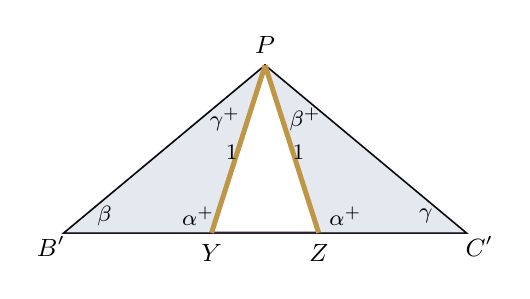
\begin{tikzpicture}[scale=0.85]
  \coordinate (P) at (0, 2.5); \coordinate (Bp) at (-3, 0); \coordinate (Cp) at (3, 0);
  
  \draw[line width=0.8pt, morleydark] (P) -- (Bp) -- (Cp) -- cycle;
  
  \coordinate (Y) at (-0.8, 0); \coordinate (Z) at (0.8, 0);
  
  \draw[fill=morleyblue!15] (P) -- (Bp) -- (Y) -- cycle;
  \draw[fill=morleyblue!15] (P) -- (Cp) -- (Z) -- cycle;
  
  \draw[line width=1.8pt, morleygold] (P) -- (Y);
  \draw[line width=1.8pt, morleygold] (P) -- (Z);
  
  \node[font=\small] at (0, 2.8) {$P$};
  \node[font=\small] at (-3.2, -0.2) {$B'$};
  \node[font=\small] at (3.2, -0.2) {$C'$};
  \node[font=\small] at (-0.8, -0.3) {$Y$};
  \node[font=\small] at (0.8, -0.3) {$Z$};
  
  \node[font=\footnotesize] at (-0.5, 1.2) {$1$}; \node[font=\footnotesize] at (0.5, 1.2) {$1$};
  
  \node[font=\footnotesize] at (-2.4, 0.25) {$\beta$};
  \node[font=\footnotesize] at (2.4, 0.25) {$\gamma$};
  \node[font=\footnotesize] at (-1, 0.25) {$\alpha^+$};
  \node[font=\footnotesize] at (1.2, 0.25) {$\alpha^+$};
  \node[font=\footnotesize] at (-.6, 1.7) {$\gamma^+$};
  \node[font=\footnotesize] at (.6, 1.7) {$\beta^+$};
\end{tikzpicture}
\end{column}
\end{columns}
\end{frame}

% =============================================
% PROOF 3: SYNTHETIC PROOF (PART 3)
% =============================================
\begin{frame}{Proof 3: Synthetic Proof (Part 3)}
\begin{columns}[T]
\begin{column}{0.5\textwidth}
\small
\textbf{Assembling the Master Triangle}
\vspace{0.1cm}

We attach the three abutting triangles to the central equilateral $\triangle PQR$. Does the spoke triangle fit into the remaining gap at the highlighted right vertex ($Q$)?

The angles meeting at $Q$ from the equilateral and abutting triangles are $60^\circ$ (or $0^+$), $\alpha^+$, and $\gamma^+$. Their sum is $60^\circ \!+\! (\alpha \!+\! 60^\circ) \!+\! (\gamma \!+\! 60^\circ) = 180^\circ \!+\! \alpha \!+\! \gamma$. Since $\alpha \!+\! \beta \!+\! \gamma \!=\! 60^\circ$, this is $240^\circ \!-\! \beta$. The remaining gap is $360^\circ \!-\! (240^\circ \!-\! \beta) \!=\! 120^\circ \!+\! \beta \!=\! \beta^{++}$. This exactly accommodates the spoke triangle $QA'C'$!

By ASA congruence ($\triangle C'QZ \cong \triangle CQP$), $C'Q \!=\! CQ$, so $C'$ is precisely the vertex $C$. Assembling all 7 pieces yields a perfect triangle $ABC$. The total angle at $C$ is $3\gamma$, proving the adjacent lines are trisectors!
\end{column}
\begin{column}{0.55\textwidth}
\centering
\begin{tikzpicture}
  \node[inner sep=0pt] (img) {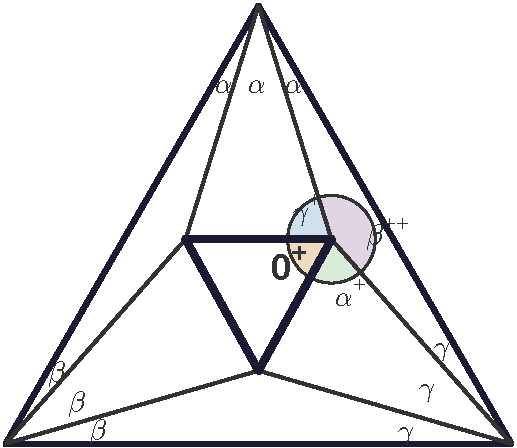
\includegraphics[width=0.65\linewidth]{figure5.pdf}};
  \node[text=morleydark, font=\bfseries] at (img.north) [yshift=-3mm] {$A$};
  \node[text=morleydark, font=\bfseries] at (img.south west) [xshift=5mm, yshift=3mm] {$B$};
  \node[text=morleydark, font=\bfseries] at (img.south east) [xshift=-5mm, yshift=3mm] {$C$};
\end{tikzpicture}
\end{column}
\end{columns}
\end{frame}

% =============================================
% PROOF 4: THE GROUP THEORY LENS
% =============================================
\begin{frame}{Proof 4: The Group Theory Lens}
\begin{columns}[T]
\begin{column}{0.48\textwidth}
\small
\textbf{The Affine Group Shift}
\vspace{0.1cm}

Connes shifts the framework from Euclidean geometry to the affine group of the line over $\mathbb{C}$.

\begin{itemize}\footnotesize
  \item \textbf{Transformations} take the form $g(x) = ax + b$, represented as matrices $g = \begin{bmatrix} a & b \\ 0 & 1 \end{bmatrix}$.
  \item \textbf{Rotations:} Let $g_1, g_2, g_3$ be rotations around $A, B, C$. The angle of each is two-thirds of the full triangle angle.
\end{itemize}
\end{column}
\begin{column}{0.48\textwidth}
\small
\textbf{Fixed Points as Intersections}
\vspace{0.1cm}

For any affine map $g(x) = ax + b$ (with $a \neq 1$), the unique fixed point is:
\[ \text{fix}(g) = \frac{b}{1-a} \]

Connes proves that the fixed points of the pairwise products $g_1g_2$, $g_2g_3$, $g_3g_1$ are precisely the trisector intersections $\alpha, \beta, \gamma$.
\end{column}
\end{columns}
\end{frame}

\begin{frame}{Proof 4: Equivalence (The Proof)}
\small
\textbf{The Algebraic Definition of an Equilateral Triangle}
\vspace{0.1cm}

Three points $\alpha, \beta, \gamma$ form an equilateral triangle iff $\alpha + j\beta + j^2\gamma = 0$ (where $j^3 = 1, j \neq 1$).

\vspace{0.1cm}
\textbf{The Crucial Computation}
\vspace{0.1cm}

Setting $g_1^3 g_2^3 g_3^3 = 1$ forces the translational component $b = 0$. Computing $b$ explicitly using $a_1 a_2 a_3 = j$ yields the factorization:

\vspace{-0.1cm}
\begin{block}{\footnotesize The Translational Part $b$}
\footnotesize
\[ b = -j a_1^2 a_2 (a_1 - j) (a_2 - j) (a_3 - j) \cdot (\alpha + j\beta + j^2\gamma) \]
\end{block}
\vspace{-0.1cm}

\textbf{Conclusion}
\vspace{0.1cm}

By hypothesis the pairwise products are not pure translations, so each $(a_k - j) \neq 0$. Since $b = 0$ is a geometric certainty ($g_1^3 g_2^3 g_3^3 = 1$ for any triangle), the remaining factor must vanish:
\[ \alpha + j\beta + j^2\gamma = 0 \]
This is the equilateral triangle condition. No diagram required.
\end{frame}

% ==============================================
% PROOF 5: THE CIRCLE INTERSECTION LENS
% ==============================================
\begin{frame}{Proof 5: The Circle Intersection Lens (Part 1)}
\begin{columns}[T]
\begin{column}{0.48\textwidth}
\small
\textbf{A New Reverse Construction}
\vspace{0.1cm}

We start with an equilateral triangle $P_1 P_2 P_3$ and angles $\alpha_1, \alpha_2, \alpha_3$ (summing to $\pi/3$). We construct a triangle with angles $3\alpha_1, 3\alpha_2, 3\alpha_3$ whose trisectors meet at $P_1, P_2, P_3$.

\vspace{0.2cm}
\textbf{The Circles and Chords}
\vspace{0.1cm}

\begin{itemize}\scriptsize
  \item Construct a circle $S_1$ through $P_2, P_3$ such that chord $P_2 P_3$ subtends angle $\alpha_1$.
  \item Find points $Q_1, R_1$ on $S_1$ such that chords $Q_1 P_3$ and $P_2 R_1$ equal $P_2 P_3$.
  \item Repeat to construct circles $S_2, S_3$ and points $Q_2, R_2, Q_3, R_3$.
  \item Let the line $Q_1 R_2$ and line $R_1 Q_3$ intersect at $X_1$. Form $X_2$ and $X_3$ similarly.
\end{itemize}
\end{column}

\begin{column}{0.5\textwidth}
\vspace{-0.5cm}
\centering
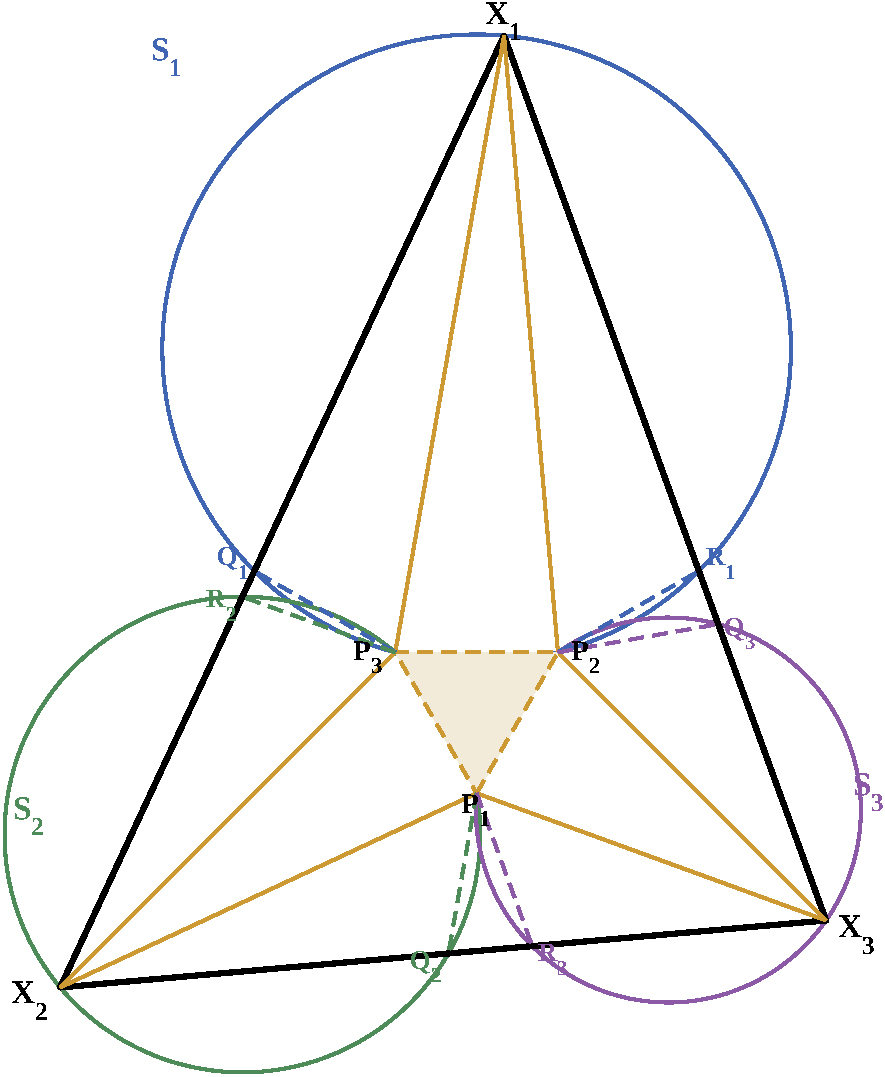
\includegraphics[width=0.65\textwidth]{figure1.pdf}
\end{column}
\end{columns}
\end{frame}
\begin{frame}{Proof 5: The Circle Intersection Lens (Part 2)}
\small
\textbf{The Pentagonal Angle Sum}
\vspace{0.1cm}

By elementary angle chasing, $P_i Q_j X_i = P_i R_j X_k = \frac{2\pi}{3} - \alpha_i$.
Summing the angles of the pentagon $P_2 Q_1 X_1 R_1 P_3$ (which must equal $3\pi$), we deduce exactly that $\angle Q_1 X_1 R_1 = 3\alpha_1$.

\vspace{0.2cm}
\textbf{Trisection on the Circle}
\vspace{0.1cm}

\begin{itemize}\footnotesize
  \item Because $\angle Q_1 X_1 R_1 = 3\alpha_1$ correctly subtends the arc on $S_1$, $X_1$ must lie exactly on the circle $S_1$.
  \item Because the chords $Q_1 P_3$, $P_3 P_2$, and $P_2 R_1$ were specifically constructed to be equal in length, they must subtend equal angles from $X_1$.
  \item Thus, the lines $X_1 P_2$ and $X_1 P_3$ cleanly \textbf{trisect} the angle $X_1$.
\end{itemize}

Repeating this symmetry for all three vertices constructs a triangle $X_1 X_2 X_3$ with angles $3\alpha_i$ correctly trisected by $P_1, P_2, P_3$, proving Morley's Theorem!
\end{frame}

\begin{frame}{Beyond the Proofs: Two More Perspectives}
\small
The five proofs above are by no means exhaustive:
\vspace{0.2cm}
\begin{itemize}
    \item \textbf{Inversive Geometry (Morley, 1899):} Morley originally studied variable cardioids tangent to a triangle's extended sides. He discovered that the \textit{centers} of these cardioids precisely track the 27 intersection points of the general angle trisectors.
    
    \vspace{0.15cm}
    
    \item \textbf{Holonomy (Differential Geometry):} Using marked similarity triangles (MSTs) around an internal vertex, we can calculate a local scale factor called \textit{holonomy}. Proving this holonomy equals 1 guarantees the geometry maps onto a flat plane perfectly, without angle gaps.
\end{itemize}
\end{frame}

\begin{frame}[plain]
\begin{tikzpicture}[remember picture,overlay]
  \fill[morleylight] (current page.south west) rectangle (current page.north east);
  \node[opacity=0.07] at (current page.center) {\begin{tikzpicture}[scale=2.5]\draw[line width=5pt,morleymain] (0,0)--(3,0)--(1.5,2.598)--cycle;\end{tikzpicture}};
\end{tikzpicture}
\vspace{1.5cm}
\begin{center}
  {\Huge\textcolor{morleymain}{\textbf{Thank You}}}\\[1.2cm]
  {\large\textcolor{morleydark!80}{\textit{``Mathematics is the art of giving the same name to different things.''}}}\\[0.2cm]
  {\large\textcolor{morleydark!80}{\textit{--- Henri Poincaré}}}\\[0.8cm]
  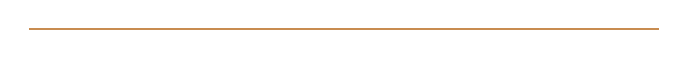
\begin{tikzpicture}
    \draw[morleyaccent, line width=0.8pt] (0,0) -- (8cm,0);
  \end{tikzpicture}\\[0.8cm]
  
\begin{tikzpicture}[scale=0.45]
    \draw[line width=1.5pt,morleygold] (0,0)--(3,0)--(1.5,2.598)--cycle;
    \foreach \x/\y in {1.0/0.58, 2.0/0.58, 1.5/1.30}{
      \fill[morleygold] (\x,\y) circle (2.5pt);
    }
  \end{tikzpicture}\\[0.4cm]
  {\footnotesize\textcolor{morleydark!50}{Sanatan Kumar Gupta \quad | \quad 19/04/2026}}
\end{center}
\end{frame}
% ===================
% REFERENCES
% ===================
\begin{frame}[allowframebreaks]{References}
\small\begin{thebibliography}{10}

\bibitem{Connes1998}
Connes, A. (1998).
\newblock A new proof of Morley’s theorem.
\newblock \emph{Publications Math\'{e}matiques de l’I.H.\'{E}.S.}, S88, 43--46.

\bibitem{Conway2005}
Conway, J. H. (2005).
\newblock The power of mathematics.
\newblock In A. F. Blackwell \& D. MacKay (Eds.), \emph{Power} (pp. 16--36). Cambridge University Press.

\bibitem{Cundy1984}
Cundy, H. M. (1984).
\newblock A direct proof of Morley’s theorem.
\newblock \emph{The Mathematical Gazette}, 68(444), 112--119.

\bibitem{Doyle2018}
Doyle, P., \& Sethi, S. (2018).
\newblock Conway’s doughnuts.
\newblock \emph{arXiv:1804.04024}.

\bibitem{Morley1900}
Morley, F. (1900).
\newblock On the metric geometry of the plane n-line.
\newblock \emph{Transactions of the American Mathematical Society}, 1, 97--115.

\bibitem{Morley1933}
Morley, F., \& Morley, F. V. (1933).
\newblock \emph{Inversive Geometry}.
\newblock Ginn and Company.

\bibitem{Newman1996}
Newman, D. J. (1996).
\newblock The Morley Miracle.
\newblock \emph{The Mathematical Intelligencer}, 18(1), 31--32.

\bibitem{Oakley1978}
Oakley, C. O., \& Baker, J. C. (1978).
\newblock The Morley Trisector Theorem.
\newblock \emph{The American Mathematical Monthly}, 85(9), 737--745.

\bibitem{Taylor1914}
Taylor, F. G., \& Marr, W. L. (1914).
\newblock The six trisectors of each of the angles of a triangle.
\newblock \emph{Proceedings of the Edinburgh Mathematical Society}, 32, 119--131.

\bibitem{Walls1944}
Walls, N. (1944).
\newblock An Elementary Proof of Morley’s Trisector Theorem.
\newblock \emph{The Mathematical Gazette}, 28(278), 12--13.

\end{thebibliography}
\end{frame}



\end{document}
